\chapter{Calcolo di autovalori e autovettori}
	
	\noindent Il calcolo degli autovalori di una data matrice quadrata \(A\) di ordine \(n\) consiste nel trovare gli \(n\) numeri \(\lambda_1, \dots, \lambda_n\) tali che esista \(x \ne \vec{0}\) tale che \(A x = \lambda_i x\) per un certo \(i \in \Set{1, \dots, n}\).
	
	È noto che gli autovalori di \(A\) sono anche gli zeri del polinomio caratteristico \(p_A (X) = \det (A - X \uno_n)\), perciò sono \(n\) numeri complessi, se contati con molteplicità.
	
	Nelle applicazioni talvolta si richiede di calcolare tutti gli autovalori di \(A\), talvolta solo alcuni -- ad esempio solo quelli di massimo modulo, in modo da determinare il raggio spettrale di \(A\).
	
\section{Teoremi di Gerschgorin}
	
	\begin{teorema}[Gerschgorin \textsc{i}]\label{th:gerschgorin-1}
		Data una matrice quadrata \(A\) di ordine \(n\) e di autovalori \(\lambda_1, \dots, \lambda_n\) e definiti per ogni \(i \in \Set{1, \dots, n}\)
		\begin{equation*}
			K_i = \Set{z \in \C : \abs{z - a_{i, i}} \le \sum_{\substack{j = 1 \\ j \ne i}}^n \abs{a_{i, j}}}
		\end{equation*}
		si verifica
		\begin{equation}\label{eq:gerschgorin-1}
			\Set{\lambda_1, \dots, \lambda_n} \subseteq \bigcup_{i = 1}^n K_i
		\end{equation}
	\end{teorema}

	\begin{esempio}\label{eg:gersch-1}
		Consideriamo la matrice
		\begin{equation*}
			A =
			\begin{pmatrix}
				15 & -2 & 2  \\
				1  & 10 & -3 \\
				-2 & 1  & 0
			\end{pmatrix}
		\end{equation*}
		I suoi cerchi di Gerschgorin sono
		\begin{align*}
			K_1 &= \Set{z \in \C : \abs{z - 15} \le 4} \\
			K_2 &= \Set{z \in \C : \abs{z - 10} \le 4} \\
			K_3 &= \Set{z \in \C : \abs{z} \le 3}
		\end{align*}
		Per il Teorema~\ref{th:gerschgorin-1}, gli autovalori di \(A\) appartengono all'unione di questi tre cerchi, come si può vedere nella Figura~\ref{fig:gersch-1}.
		
		\begin{figure}[tpb]
			\centering
			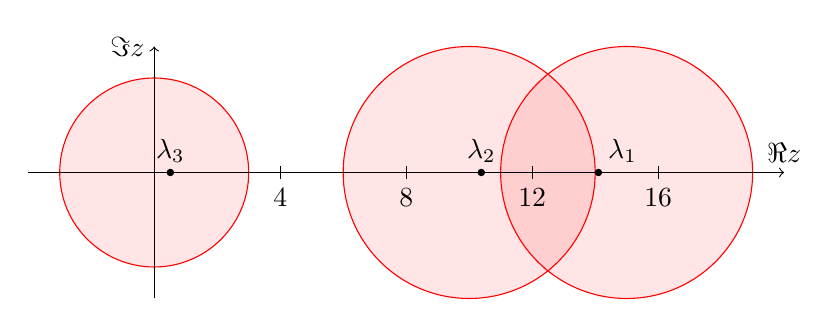
\begin{tikzpicture}[scale=0.4]
				\filldraw[color = red, fill opacity = 0.1] (15,0) circle[radius=4];
				\filldraw[color = red, fill opacity = 0.1] (10,0) circle[radius=4];
				\filldraw[color = red, fill opacity = 0.1] (0,0) circle[radius=3];
				\filldraw (14.1026,0) circle[radius=0.1] node [above right] {\(\lambda_1\)};
				\filldraw (10.3854,0) circle[radius=0.1] node [above] {\(\lambda_2\)};
				\filldraw (0.512085,0) circle[radius=0.1] node [above] {\(\lambda_3\)};
				\draw[->] (-4,0) -- (20,0) node [above] {\(\Re z\)};
				\draw[->] (0,-4) -- (0,4) node [left] {\(\Im z\)};
				\foreach \i in {4, 8, 12, 16} {
					\draw (\i, 0.2) -- (\i, -0.2) node [below] {\i};	
				}
			\end{tikzpicture}
			
			\caption{Rappresentazione dei cerchi di Gerschgorin e degli autovalori relativi alla matrice \(A\) dell'Esempio~\ref{eg:gersch-1}.}\label{fig:gersch-1}
		\end{figure}
	\end{esempio}

	\begin{teorema}[Gerschgorin \textsc{ii}]\label{th:gerschgorin-2}
		Se l'unione \(M_1\) di \(k\) cerchi di Gerschgorin è disgiunta dall'unione \(M_2\) dei rimanenti \(n - k\) cerchi, allora \(M_1\) contiene esattamente \(k\) autovalori di \(A\) contati con molteplicità e \(M_2\) contiene esattamente \(n - k\) autovalori di \(A\) contati con molteplicità.
	\end{teorema}

	Guardando la Figura~\ref{fig:gersch-1}, è evidente che la matrice \(A\) dell'Esempio~\ref{eg:gersch-1} abbia un solo autovalore in \(K_1\) e due autovalori in \(K_2 \cup K_3\).
	
	\begin{definizione}
		Una matrice quadrata \(A\) di ordine \(n \ge 2\) si dice \emph{riducibile} se esistono una matrice di permutazione \(P\) e un intero \(k \in \Set{1, \dots, n - 1}\) tali che
		\begin{equation}
			P \! A \tra{P} =
			\begin{pmatrix}
				A_{1, 1} & A_{1, 2} \\
				\zero    & A_{2, 2}
			\end{pmatrix}
		\end{equation}
		con \(A_{1, 1} \in M_k (\C)\) e \(A_{2, 2} \in M_{n - k} (\C)\).
		
		Una matrice quadrata si dice \emph{irriducibile} se non è riducibile.
	\end{definizione}

	Per verificare che una matrice sia irriducibile, ricordiamo che una matrice quadrata \(A\) è irriducibile se e solo se il suo grafo orientato associato è fortemente connesso, ovvero se e solo se per ogni coppia \((i, j)\) esiste un cammino da \(i\) verso \(j\).\footnote{A partire da una matrice quadrata \(A\) di ordine \(n\) se ne costruisce il grafo orientato associato ponendo \(1, \dots, n\) come nodi e tracciando il lato \((i, j)\) se e solo se \(a_{i, j} \ne 0\).} Nella Figura~\ref{fig:grafo-gersch-1} è rappresentato il grafo orientato associato alla matrice \(A\) dell'Esempio~\ref{eg:gersch-1}: in base ad esso, si può affermare che \(A\) è irriducibile.
	
	\begin{figure}[tpb]
		\centering
		
		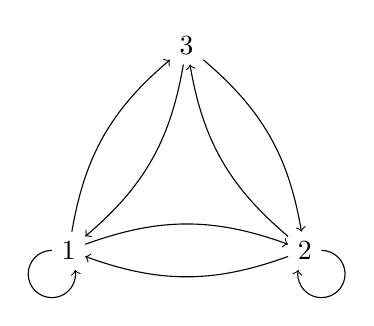
\begin{tikzpicture}[scale = 3]
			\node (a) at (0,0) {1};
			\node (b) at (1,0) {2};
			\node (c) at (0.5,0.866) {3};
			
			\draw[->] (a) to[bend left = 20] (b);
			\draw[->] (a) to[bend left = 20] (c);
			\draw[->] (b) to[bend left = 20] (a);
			\draw[->] (b) to[bend left = 20] (c);
			\draw[->] (c) to[bend left = 20] (a);
			\draw[->] (c) to[bend left = 20] (b);
			
			\draw[->] (a.west) arc[start angle = 90, end angle = 370, radius = 1mm];
			\draw[->] (b.east) arc[start angle = 90, end angle = -190, radius = 1mm];
		\end{tikzpicture}
	
		\caption{Grafo orientato associato alla matrice \(A\) dell'Esempio~\ref{eg:gersch-1}.}\label{fig:grafo-gersch-1}
	\end{figure}

	\begin{teorema}[Gerschgorin \textsc{iii}]\label{th:gerschgorin-3}
		Se una matrice quadrata \(A\) di ordine \(n\) è irriducibile e un suo autovalore \(\lambda\) appartiene alla frontiera dell'unione dei cerchi di Gerschgorin di \(A\), allora \(\lambda\) appartiene alla frontiera di ogni cerchio di Gerschgorin di \(A\).
	\end{teorema}

	\begin{esempio}\label{eg:gersch-2}
		Consideriamo la matrice
		\begin{equation*}
			B =
			\begin{pmatrix}
				2  & -1 & 0  & 0  \\
				-1 & 2  & -1 & 0  \\
				0  & -1 & 2  & -1 \\
				0  & 0  & -1 & 2
			\end{pmatrix}
		\end{equation*}
		Essa è irriducibile, come mostra il suo grafo orientato nella Figura~\ref{fig:grafo-gersch-2}. Per il Teorema~\ref{th:gerschgorin-1} tutti gli autovalori di \(B\) appartengono alla palla chiusa di centro \(2\) e raggio \(2\), ma non possono appartenere contemporaneamente alle frontiere di tutti i cerchi di Gerschgorin; per questo motivo, dal Teorema~\ref{th:gerschgorin-3} segue che \(B\) è non singolare.
		
		\begin{figure}[tpb]
			\centering
			
			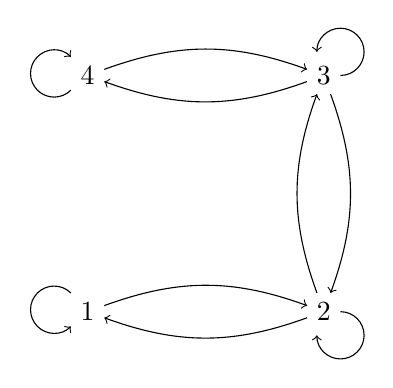
\begin{tikzpicture}[scale = 3]
				\node (a) at (0,0) {1};
				\node (b) at (1,0) {2};
				\node (c) at (1,1) {3};
				\node (d) at (0,1) {4};
				
				\draw[->] (a) to[bend left = 20] (b);
				\draw[->] (b) to[bend left = 20] (a);
				\draw[->] (b) to[bend left = 20] (c);
				\draw[->] (c) to[bend left = 20] (b);
				\draw[->] (c) to[bend left = 20] (d);
				\draw[->] (d) to[bend left = 20] (c);
				
				\draw[->] (a.north west) arc[start angle = 45, end angle = 315, radius = 1mm];
				\draw[<-] (d.north west) arc[start angle = 45, end angle = 315, radius = 1mm];
				\draw[->] (b.east) arc[start angle = 90, end angle = -180, radius = 1mm];
				\draw[->] (c.east) arc[start angle = -90, end angle = 180, radius = 1mm];
			\end{tikzpicture}
			
			\caption{Grafo orientato associato alla matrice \(B\) dell'Esempio~\ref{eg:gersch-2}.}\label{fig:grafo-gersch-2}
		\end{figure}
	\end{esempio}

	\begin{osservazione}
		Poiché \(\tra{A}\) ha gli stessi autovalori di \(A\), è possibile raffinare il criterio dei cerchi di Gerschgorin affermando che gli autovalori di \(A\) appartengono all'intersezione tra l'unione dei cerchi di Gerschgorin di \(A\) e l'unione dei cerchi di Gerschgorin di \(\tra{A}\).
	\end{osservazione}

\section{Metodo delle potenze}
	
	\noindent Il metodo delle potenze si usa per calcolare l'autovalore di massimo modulo di una matrice quadrata. Nel nostro caso supporremo sempre che la matrice \(A\) sia quadrata, di ordine \(n\), diagonalizzabile e tale che i suoi autovalori \(\lambda_1, \dots, \lambda_n\) verifichino\(\abs{\lambda_1} > \abs{\lambda_2} \ge \dots \ge \abs{\lambda_n}\).
	
	Ricordiamo che una matrice quadrata \(A\) di ordine \(n\) è diagonalizzabile se e solo se ammette \(n\) autovettori linearmente indipendenti. Ricordiamo anche che, se \(A\) ammette \(n\) autovalori distinti, allora è diagonalizzabile; se \(A\) è simmetrica o hermitiana, allora è diagonalizzabile.
	
	\begin{teorema}\label{th:metodo-potenze-converge}
		Data una matrice \(A \in M_n (\C)\) diagonalizzabile e con autovalori \(\lambda_1, \dots, \lambda_n\) tali che \(\abs{\lambda_1} > \abs{\lambda_2} \ge \dots \ge \abs{\lambda_n}\) e scelti \(u_1, \dots, u_n \in \C^n \setminus \Set{\vec{0}}\) tali che \(A u_k = \lambda_k u_k\) per ogni \(k \in \Set{1, \dots, n}\), se il vettore \(y_0 = \sum_{k = 1}^n \alpha_k u_k\) verifica \(\alpha_1 \ne 0\), allora la successione \((y_s)_{s \in \N}\) definita da
		\begin{equation}
			y_{s + 1} = A y_s
		\end{equation}
		per ogni \(s \in \N\) converge per direzione alla direzione di \(u_1\) e il \emph{quoziente di Rayleigh}
		\begin{equation}
			\rayleigh (y_s, A) = \frac{(A y_s, y_s)}{(y_s, y_s)}
		\end{equation}
		converge a \(\lambda_1\).
	\end{teorema}